
\newpage
\section*{Appendix: System GMM estimator}
\label{systemGMM}
\addcontentsline{toc}{section}{Appendix: System GMM estimator}

We estimate a dynamic panel data model by using the System GMM estimator developed by Arellano and Bover (1995) and Blundell and Bond (1998) based on the Difference GMM estimator proposed earlier by Holtz-Eakin et al. (1988) and Arellano and Bond (1991). Both, Difference and System GMM estimators are specific applications of the generalized-method-of-moments (Hansen, 1982). In this section we explain the underlying details of the estimator in five steps. First, we outline a simple autoregressive panel data model and review inconsistency issues of common estimators. Second, considering the same simple autoregressive model, we explain the Difference GMM estimator. Third, we go further to construct the System GMM estimator. Fourth, we extend the explanation to multivariate models. Finally, we outline some issues about the conditions for optimality of the System GMM estimator and relevant tests. In most of the explanation we follow rigorous surveys of Difference and System GMM estimators made by Arellano and Honore (2001), Blundell et al. (2000) and Bond (2002).

\subsection*{Biases of standard panel data estimators}

We consider a simple autoregressive panel data model of the form:
\begin{equation}
\label{modelar}
\tag{1'}
\begin{aligned}
y_{it}&=\alpha y_{it-1} + \varepsilon_{it}\\
\varepsilon_{it}&=\mu _{i}+v_{it}
\end{aligned}
\end{equation}
where the following assumptions hold for the structure of the fixed effect and the idiosyncratic shock:
\begin{equation}
\label{as1}
\tag{2'}
E\left[\mu_{i}\right]=E\left[v_{i}\right]=E\left[\mu_{i}v_i\right]=0\text{; for $i=1,...,N$ and $t=2,...,T$}
\end{equation}
and
\begin{equation}
\label{as2}
\tag{3'}
E\left[v_{it}v_{is}\right]=0\text{; for $i=1,...,N$ and $\forall t\neq s$}
\end{equation}

Additionally, a further assumption regarding the initial conditions is also valid (Ahn and Schmidt, 1995):

\begin{equation}
\label{as3}
\tag{4'}
E\left[y_{i1}v_{it}\right]=0\text{; for $i=1,...,N$ and $t=2,...,T$}
\end{equation}

The introduction of a lag of the dependent variable in (\ref{model}) yields asymptotic bias in standard estimators such as OLS and Fixed Effects, which are both biased and inconsistent (see Baltagi (2008) and Blundell et al. (2000) for further details). In the OLS case, since $y_{it}$ is a function of $\mu_{i}$, $y_{it-1}$ is also a function of $\mu_{i}$ and thus it is correlated with the error term. Furthermore, in the case of the Fixed Effects estimator, the within transformation removes the fixed effects by taking the equation in levels $y_{it}=\alpha y_{it-1} + \mu_i+v_{it}$ and subtracting out the average over time $\bar y_{i.}=\alpha \bar y_{i.-1} +\mu_i +\bar v_{i.}$. The resulting model is of the form $(y_{it}-\bar y_{i.})=\alpha (y_{it-1}-\bar y_{i.-1})+ (v_{it}-\bar v_{i.})$. However, the idiosyncratic shock $v_{it-1}$ is correlated with $y_{it-1}$ and therefore in the transformed model $(y_{it-1}-\bar y_{i.-1})$ will be correlated with $(v_{it}-\bar v_{i.})$ (Nickel, 1981).

Under an additional restriction of \emph{covariance stationarity}\footnote{\emph{Covariance stationarity} requires further assumptions on the structure of the error components, namely $E[v_{it}^2]=\sigma_v^2$ for $i=1,...,N$ and $E[\lambda_{i1}^2]=\sigma_v^2 / (1-\alpha^2)$ for $i=1,...,N$, $t=2,...,T$ where $\lambda_{i1}$ is such that the process is \emph{mean stationary} with $y_{i1}=\mu_{i}/(1-\alpha)+\lambda_{i1}$} the asymptotic bias of the OLS estimator is given by (Blundell et al., 2000; Sevestre and Trognon, 1985):
\[
\text{plim}\left(\hat\alpha_{OLS}-\alpha \right) =\left(1-\alpha\right)\frac{E[\mu_i^2]/E[v_{it}^2]}{E[\mu_i^2]/E[v_{it}^2]+\frac{1-\alpha}{1+\alpha}}
\]
and respectively, the asymptotic bias of the Fixed Effects estimator is (Nickel, 1981):
\[
\text{plim}\left(\hat\alpha_{FE}-\alpha \right)=-\frac{\frac{1+\alpha}{T-1}\left(1-\frac{1-\alpha^T}{T(1-\alpha)}\right)}{1-\frac{2\alpha}{(1-\alpha)(T-1)}\left(1-\frac{1-\alpha^T}{T(1-\alpha)}\right)}
\]

\subsection*{Difference GMM estimator}

The autoregressive panel data model described by (\ref{modelar}) to (\ref{as3}) imply the following $0.5(T-1)(T-2)$ orthogonality conditions, which are equivalent to those given by (\ref{momentsDiff}) in the paper except for the exclusion of other covariates different than the lag of the dependent variable:

\begin{equation}
\label{momentsDiffAp}
\tag{5'}
E\left[ y_{it-s}\Delta \varepsilon_{it}\right]=0 \text{; for $t=3,...,T$, $2\leq s \leq t-1$}
\end{equation}

The usefulness of these orthogonality conditions is straightforward when looking at the first-difference transformation of the model, aimed at eliminating the fixed effects. This is done by multiplying (\ref{modelar}) by $\mathbf{I}_N \otimes \mathbf{M}_{\Delta}$ with $\mathbf{I}_N$ being an identity matrix of order $N$ and $\mathbf{M}_{\Delta}$ a matrix with diagonal of $-1s$ and a sub-diagonal of $1s$ to the right. The transformation yields a model of the form\footnote{An alternative to first-differencing is the forward-orthogonal-deviations transformation in which the fixed effects are removed by subtracting the average of all available future observations instead of the previous one (Arellano and Bover, 1995). This alternative yields better results whenever there are gaps in unbalanced panels}:
\[
\Delta y_{it}=\alpha \Delta y_{it-1} +\Delta v_{it}
\]

The conditions in (\ref{momentsDiffAp}) can also be expressed as:

\begin{equation*}
E\left[ \mathbf{Z}'_{di}\mathbf{\Delta \varepsilon}_{i}\right]=0
\end{equation*}
where $\mathbf{\Delta \varepsilon}_{i}$ is the $T-2$ vector $(\Delta \varepsilon_{i3},\Delta \varepsilon_{i4},...,\Delta \varepsilon_{iT})'$ and $\mathbf{Z}_{di}$ is the $(T-2)\times 0.5(T-1)(T-2)$ instruments matrix given by:
\[
\mathbf{Z}_{di} = \left[ {\begin{array}{*{20}{c}}
{{y_{i1}}}&0&0&{...}&0&{...}&0\\
0&{{y_{i1}}}&{{y_{i2}}}&{...}&0&{...}&0\\
.&.&.&{...}&.&{...}&.\\
0&0&0&{...}&{{y_{i1}}}&{...}&{{y_{iT - 2}}}
\end{array}} \right]
\]
or, when collapsing the matrix in order to reduce the instrument count, $\mathbf{Z}_{di}$ becomes a $(T-2)\times (T-2)$ matrix given by:
\[
\mathbf{Z}_{di} = \left[ {\begin{array}{*{20}{c}}
{{y_{i1}}}&0&{...}&0\\
{{y_{i1}}}&{{y_{i2}}}&{...}&0\\
.&.&{...}&.\\
{{y_{i1}}}&{{y_{i2}}}&{...}&{{y_{iT - 2}}}
\end{array}} \right]
\]

The Difference GMM estimator solves:
\[
{{\hat \alpha }_{diff - GMM}} = \mathop {\arg \min }\limits_{\alpha  \in \Re } \mathbf{\Delta \varepsilon}' \mathbf{Z}_{d}{\mathbf{W}_{N}^d}\mathbf{Z}'_{d}\mathbf{\Delta \varepsilon} 
\]
for some symmetric, positive semi definite matrix $\mathbf{W}_{N}^d$, $\mathbf{Z}'_{d}$ the $0.5(T-1)(T-2)\times N(T-2)$ instruments matrix $(\mathbf{Z}'_{d1},\mathbf{Z}'_{d2},...,\mathbf{Z}'_{dN})$ or its $(T-2)\times N(T-2)$ collapsed counterpart and $\mathbf{\Delta \varepsilon}'$ the $N(T-2)$ vector $(\mathbf{\Delta \varepsilon}'_1,\mathbf{\Delta \varepsilon}'_2,...,\mathbf{\Delta \varepsilon}'_N)$. Finally, by letting $\mathbf{\Delta y}$ and $\mathbf{\Delta y}_{-1}$ be $N(T-2)$ vectors constructed in the same way as $\mathbf{\Delta \varepsilon}$ by stacking the $T-2$ vectors $\mathbf{\Delta y}'_i=(\Delta y_{i3},\Delta y_{i4},...,\Delta y_{iT})$ and $\mathbf{\Delta y}'_{i,-1}=(\Delta y_{i2},\Delta y_{i4},...,\Delta y_{iT-1})$ respectively across individuals, the estimator for $\alpha$ takes the form:
\[
{{\hat \alpha }_{diff - GMM}} = {\left( \mathbf{\Delta y}'_{-1}\mathbf{Z}_d \mathbf{W}_{N}^d \mathbf{Z}'_d \mathbf{\Delta y}_{-1} \right)^{ - 1}} \mathbf{\Delta y}'_{-1}\mathbf{Z}_d \mathbf{W}_{N}^d \mathbf{Z}'_d \mathbf{\Delta y} 
\]

The optimal two-step generalized-method-of-moments estimation is achieved with a choice of the weighting matrix $\mathbf{W}_{N}^d$ given by:
\[
\mathbf{W}_{N}^d=\left( \frac{1}{N} \sum\limits_{i=1}^{N} \mathbf{Z}'_{di} \hat{ \mathbf{\Delta \varepsilon}_i} \hat{ \mathbf{\Delta \varepsilon}'_i} \mathbf{Z}_{di} \right)^{-1}
\]

The first step comprises on using an identity weighting matrix to estimate $\hat \alpha$ consistently. Then, in a second step, the residuals from this estimation (i.e. $\hat{\mathbf{\Delta \varepsilon}_i}$) are used in the optimal choice of $\mathbf{W}_{N}^d$. This renders the two-step estimation of $ \alpha$.

\subsection*{System GMM estimator}

We now consider an additional assumption by imposing a restriction on the initial conditions process generating $y_{i1}$ (Arellano and Bover, 1995; Blundell and Bond, 1998):
\begin{equation}
\label{as4}
\tag{6'}
E\left[\Delta y_{i2}\mu_{i}\right]=0\text{; for $i=1,...,N$}
\end{equation}

Together with (\ref{modelar}) to (\ref{as3}), assumption (\ref{as4}) imply an additional set of $T-2$ orthogonality conditions given by:
\begin{equation}
\label{momentsSysAp}
\tag{7'}
E\left[\Delta y_{it-1} \varepsilon_{it}\right]=0 \text{; for $t=3,...,T$}
\end{equation}

As in the case for the Difference GMM estimator, the conditions in (\ref{momentsSysAp}) can be expressed as:
\begin{equation*}
E\left[ \mathbf{Z}'_{li}\mathbf{ \varepsilon}_{i}\right]=0
\end{equation*}
where $\mathbf{\varepsilon}_{i}$ is the $T-2$ vector $( \varepsilon_{i3}, \varepsilon_{i4},..., \varepsilon_{iT})'$ and $\mathbf{Z}_{li}$ is the $(T-2)\times (T-2)$ instruments matrix given by:
\[
\mathbf{Z}_{li} = 
\left[ {\begin{array}{*{20}{c}}
{\Delta {y_{i2}}}&0&{...}&0\\
0&{\Delta {y_{i3}}}&{...}&0\\
.&.&{...}&.\\
0&0&{...}&{\Delta {y_{iT - 1}}}
\end{array}} \right]
\]
or, when collapsing the matrix in order to reduce the instrument count, $\mathbf{Z}_{li}$ becomes a $T-2$ column vector such that:
\[
\mathbf{Z}_{li} = 
\left[ {\begin{array}{*{20}{c}}
{\Delta {y_{i2}}}\\
{\Delta {y_{i3}}}\\
{...}\\
{\Delta {y_{iT - 1}}}
\end{array}} \right]
\]

Blundell and Bond (1998) propose to exploit jointly the moments conditions in (\ref{momentsDiffAp}) and (\ref{momentsSysAp}). To do so, the dataset is stacked with transformed and untransformed observations by multiplying it by $\mathbf{M}=\left(\mathbf{M}_{\Delta}\;\;\mathbf{I}\right)'$. This yields an augmented dataset of the form $ \mathbf{Y}_{i}=\left(\mathbf{\Delta} \mathbf{y}_{i}\;\;\mathbf{y}_i\right)'$ for each individual $i$, where $\mathbf{M}_{\Delta}$ is the matrix used in the first-difference transformation, a matrix with diagonal of $-1s$ and a sub-diagonal of $1s$ to the right. 

By letting $\mathbf{E}_i$ be $\left(\mathbf{\Delta} \mathbf{\varepsilon}_{i}\;\;\mathbf{\varepsilon}_i\right)'$, conditions (\ref{momentsDiffAp}) and (\ref{momentsSysAp}) can be expressed as a system of equations of the form:
\begin{equation*}
E\left[ \mathbf{Z}'_{i}\mathbf{E}_{i}\right]=0
\end{equation*}
where $\mathbf{Z}_{i}$ considers both sets of instruments corresponding to (\ref{momentsDiffAp}) and (\ref{momentsSysAp}) respectively and so it is defined by the $2(T-2)\times (T-2)(0.5(T-1)+1)$ matrix:
\[{\mathbf{Z}_i} = \left[ {\begin{array}{*{20}{c}}
{{\mathbf{Z}_{di}}}&0\\
0&{{\mathbf{Z}_{li}}}
\end{array}} \right]\]

The two-step System GMM estimator is then analogous to the one described for the Difference GMM. It solves:
\[
{{\hat \alpha }_{sys - GMM}} = \mathop {\arg \min }\limits_{\alpha  \in \Re } \mathbf{E}' \mathbf{Z}{\mathbf{W}_{N}^s}\mathbf{Z}'\mathbf{E} 
\]
for some symmetric, positive semi definite weighting matrix $\mathbf{W}_{N}^s$, $\mathbf{Z}'$ the $(T-2)(0.5(T-1)+1)\times 2N(T-2)$ or its $(T-1)\times 2N(T-2)$ counterpart for collapsed instruments matrix $(\mathbf{Z}'_{1},\mathbf{Z}'_{2},...,\mathbf{Z}'_{N})$ and $\mathbf{E}'$ the $N(T-2)$ vector $(\mathbf{E}'_1,\mathbf{E}'_2,...,\mathbf{E}'_N)$. The System GMM estimator is given by:
\[
{{\hat \alpha }_{sys - GMM}} = {\left( \mathbf{Y}'_{-1}\mathbf{Z} \mathbf{W}_{N}^s \mathbf{Z}' \mathbf{Y}_{-1} \right)^{ - 1}} \mathbf{Y}'_{-1}\mathbf{Z} \mathbf{W}_{N}^s \mathbf{Z}' \mathbf{Y} 
\]
where $\mathbf{Y}$ and $\mathbf{Y}_{-1}$ are $N(T-2)$ vectors constructed as $\mathbf{\Delta y}$ and $\mathbf{\Delta y}_{-1}$ for the Difference GMM estimator.

Finally, the optimal two-step System GMM is obtained with a choice of the weighting matrix $\mathbf{W}_{N}^s$ given by:
\[
\mathbf{W}_{N}^s=\left( \frac{1}{N} \sum\limits_{i=1}^{N} \mathbf{Z}'_{i} \hat{ \mathbf{E}_i} \hat{ \mathbf{E}'_i} \mathbf{Z}_{i} \right)^{-1}
\]
where the residuals $\hat{ \mathbf{E}_i}$ are obtained from a first-step consistent estimation of $\alpha$.

%Central Limit Theorems?

\subsection*{Multivariate models}

We now move to an autoregressive panel data model of the form:
\begin{equation}
\label{modelarmul}
\tag{8'}
\begin{aligned}
y_{it}&=\alpha y_{it-1} + \beta x_{it} + \varepsilon_{it}\\
\varepsilon_{it}&=\mu _{i}+v_{it}
\end{aligned}
\end{equation}
where $\mu _{i}$ and $v_{it}$ satisfy (\ref{as1}) to (\ref{as3}).

In addition to the orthogonality conditions given by (\ref{momentsDiffAp}) and (\ref{momentsSysAp}), which remain valid, the presence of further explanatory variables in the model allows to increase the number of moment conditions depending on whether the $x_{it}$ process is strictly exogenous, predetermined or endogenous (see Blundell et al. (2000) for additional details). Recall the $x_{it}$ process is exogenous if:
\begin{equation}
\label{ruleexo}
\tag{9'}
E\left[x_{is}v_{it}\right]=0\text{; for $s=1,...,T$; $t=2,...,T$,}
\end{equation}
it is predetermined (or weakly exogenous) if:
\begin{equation}
\label{rulepre}
\tag{10'}
\begin{aligned}
E\left[x_{is}v_{it}\right]&=0\text{; for $s=1,...,T$; $t=2,...,T$}\\
E\left[x_{is}v_{it}\right]&\neq 0\text{; for $s=t+1,...,T$; $t=2,...,T$}
\end{aligned}
\end{equation}
and it is endogenous if:
\begin{equation}
\label{ruleend}
\tag{11'}
\begin{aligned}
E\left[x_{is}v_{it}\right]&=0\text{; for $s=1,...,t-1$; $t=2,...,T$}\\
E\left[x_{is}v_{it}\right]&\neq 0\text{; for $s=t,...,T$; $t=2,...,T$}
\end{aligned}
\end{equation}

The additional orthogonality conditions are implied by a combination of the errors component structure given by (\ref{as1}) to (\ref{as3}) and respectively (\ref{ruleexo}), (\ref{rulepre}) and (\ref{ruleend}). For the first-difference transformation of the model, if the $x_{it}$ process is strictly exogenous, the additional moment conditions are:
\begin{equation}
\label{momentsDiffexo}
\tag{12'}
E\left[x_{is}\Delta \varepsilon_{it}\right]=0 \text{; for $t=3,...,T$ and $1\leq s \leq T$,}
\end{equation}
on the other hand, if the $x_{it}$ process is predetermined:
\begin{equation}
\label{momentsDiffpre}
\tag{13'}
E\left[x_{it-s}\Delta \varepsilon_{it}\right]=0 \text{; for $t=3,...,T$ and $1\leq s\leq t-1$,}
\end{equation}
and if the $x_{it}$ process is endogenous, the respective additional orthogonality conditions are:
\begin{equation}
\label{momentsDiffend}
\tag{14'}
E\left[x_{it-s}\Delta \varepsilon_{it}\right]=0 \text{; for $t=3,...,T$ and $2\leq s \leq t-1$}
\end{equation}

Likewise, there are additional moment conditions for the equation in levels. If the $x_{it}$ process is strictly exogenous or predetermined, these conditions are:
\begin{equation}
\label{momentsSysexopre}
\tag{15'}
E\left[\Delta x_{it}\varepsilon_{it}\right]=0 \text{; for $t=2,...,T$,}
\end{equation}
and if the $x_{it}$ process is endogenous:
\begin{equation}
\label{momentsSysend}
\tag{16'}
E\left[\Delta x_{it-1}\varepsilon_{it}\right]=0 \text{; for $t=3,...,T$}
\end{equation}

\subsection*{Optimal GMM and relevant tests}

Although the Difference and System GMM estimators are both consistent under (\ref{momentsDiffAp}), (\ref{momentsSysAp}) and (\ref{momentsDiffexo}) to (\ref{momentsSysend}), provided the orthogonality conditions in (\ref{momentsSysAp}), (\ref{momentsSysexopre}) and (\ref{momentsSysend}) are valid,  System GMM is more efficient than Difference GMM. This issue has been supported with Montecarlo simulations studying the finite sample behavior of both estimators (see Blundell and Bond (1998), Blundell et al. (2000) for further details). The main reason for this gain in efficiency is that when explanatory variables show persistence or the number of time series observations is small relative to the number of individuals, the set of instruments of the Difference GMM estimator becomes weak since past levels of the variables carry out little information about future changes. Therefore, the informative power of additional instruments in the System GMM estimator takes relevance when performing the estimation (Arellano and Bover, 1995; Blundell and Bond, 1998; Blundell et al., 2000).

Furthermore, the validity of the additional moment conditions given by (\ref{momentsSysAp}), (\ref{momentsSysexopre}) and (\ref{momentsSysend}) can be regarded as an empirical issue as they correspond to overidentifying restrictions (Blundell and Bond, 1998). Therefore, the choice of System over Difference GMM needs to be substantiated with overidentification tests not only for the full set of instruments but for the suspicious set of instruments included in the System GMM estimation as well. Hence the Hansen and Difference-in-Hansen tests, specifying the latter so as to focus exclusively on the extra moment conditions, are of remarkable importance when assessing the use of the System GMM estimator and both tests should be reported in every estimation obtained by using this approach. In particular, section \ref{overid} of the paper discusses the robustness of my results according to overidentifying restrictions.

On the other hand, the presence of serial autocorrelation in the idiosyncratic disturbance term $v_{it}$ renders some specific lags, both levels and differences, invalid as instruments (Arellano and Bond, 1991). As pointed out by Roodman (2009b), the full disturbance term $\varepsilon_{it}$ is presumed to be autocorrelated since it contains the individual specific effect $\mu_i$, which is handled by the design of the Difference and System GMM estimators. However, if for instance the idiosyncratic disturbances exhibit serial autocorrelation of order $1$, then the first lag of the endogenous variable $y_{it-1}$, i.e. $y_{it-2}$ is also endogenous. To control for this situation, Arellano and Bond (1991) develop a test for serial autocorrelation of the idiosyncratic disturbance aside from the fixed effects. Specifically, the test is applied to residuals of the equations in differences. Hence, the validity of lags $2$ and further as instruments for endogenous variables requires no serial autocorrelation of order $2$. All results in section \ref{results} report Arellano and Bond (1992) tests for serial correlation of order $1$ and $2$ for all estimates and support the specification of the model as discussed in detail in section \ref{auto}.

Moreover, a relevant issue to consider when following the generalized-method-of-moments approach is instrument proliferation. This is particularly important in the Difference or System GMM estimators as the number of instruments tends to increase largely. A first concern is a bias in coefficient estimates because instruments over-fit instrumented variables (Ziliak, 1997; Windmeijer, 2005). Second, Andersen and S\o rensen (1996) and Bowsher (2002) show that a large number of instruments undermines the Hansen test of overidentification restrictions by increasing the likelihood of false-positive results. There are two main techniques used to reduce the instrument count and overcome these difficulties. Either to use some out of all available lags as instruments or to combine them by collapsing the instruments matrix without dropping any lags to retain more information. Roodman (2009b) provides evidence in favor of the second alternative by using Montecarlo simulations. Collapsing the instruments matrix has been increasingly used in empirical studies and therefore we apply this technique in all estimations (see for instance Christiaensen et al. (2011), Heid et al. (2012) and Beck and Levine (2004) for applications using System GMM estimators).

A final concern is related to a severe downward bias in standard errors when performing the two-step generalized-method-of-moments estimation in small samples. The reason for this bias is that the estimated variance does not take into consideration an extra variation due to the parameters used in the first-step weighting matrix (Windmeijer, 2005). This issue can be handled by implementing a correction proposed by Windmeijer (2005) in which the extra variation is estimated to adjust the variance. All results reported in section \ref{results} include the Windmeijer (2005) correction.

\newpage


\begin{table}[p]\centering\scriptsize
\def\sym#1{\ifmmode^{#1}\else\(^{#1}\)\fi}
\caption{Summary statistics by year for time-varying variables}
\label{ds_tvar}
\begin{threeparttable}
\begin{tabular}{p{3cm}*{9}{c}}
\hline\hline
                    &        2000&        2001&        2002&        2003&        2004&        2005&        2006&        2007&        2008\\
\hline
Proportion of coca fields per 1,000 hectares&       0.821&       0.561&       0.302&       0.315&       0.322&       0.317&       0.316&       0.417&       0.325\\
                    &     [8.899]&     [5.524]&     [1.738]&     [1.493]&     [1.468]&     [1.478]&     [1.619]&     [2.044]&     [1.496]\\
Informality index land property&       0.211&       0.210&       0.205&       0.201&       0.193&       0.194&       0.187&       0.183&       0.179\\
                    &     [0.230]&     [0.228]&     [0.223]&     [0.221]&     [0.216]&     [0.216]&     [0.212]&     [0.206]&     [0.202]\\
Municipal development index&      35.006&      35.210&      34.990&      34.394&      34.515&      34.754&      57.802&      55.593&      66.955\\
                    &     [9.487]&     [9.879]&     [9.300]&     [9.309]&     [9.321]&     [9.430]&    [10.338]&     [9.026]&    [12.269]\\
Homicide rate per 100,000 inhabitants&      52.181&      55.596&      60.117&      52.822&      44.634&      39.857&      40.420&      39.826&      33.888\\
                    &    [69.218]&    [64.669]&    [75.685]&    [65.447]&    [55.183]&    [49.444]&    [50.083]&    [46.164]&    [41.373]\\
Public expenditures per capita in education&      51.323&      49.253&      57.116&      42.761&      35.903&      45.098&      42.568&      59.519&      64.975\\
                    &    [43.038]&    [46.243]&    [55.486]&    [43.535]&    [48.243]&    [60.184]&    [59.299]&    [82.215]&    [79.456]\\
Public expenditures per capita in health&      39.020&      63.890&      86.151&      48.090&      51.736&     136.599&     119.927&     159.838&     212.109\\
                    &    [37.763]&    [51.163]&    [45.835]&    [55.508]&    [58.725]&    [57.089]&    [59.081]&    [73.123]&    [77.345]\\
Public expenditures per capita in justice&       0.841&       0.548&       2.248&      15.545&      12.451&       3.982&       4.250&       6.721&       8.196\\
                    &     [3.523]&     [2.193]&     [4.647]&    [49.672]&    [20.628]&    [10.938]&     [9.435]&    [17.220]&    [14.786]\\
Number of agricultural loans per 1,000 inhabitants&       2.152&       1.817&       2.953&       4.548&       7.488&      11.473&      13.189&      12.877&      11.838\\
                    &     [3.787]&     [3.148]&     [4.247]&     [6.022]&     [9.879]&    [13.777]&    [15.892]&    [15.625]&    [14.330]\\
Land quality Gini index&       0.687&       0.688&       0.688&       0.687&       0.690&       0.690&       0.690&       0.691&       0.692\\
                    &     [0.113]&     [0.109]&     [0.108]&     [0.107]&     [0.106]&     [0.106]&     [0.105]&     [0.105]&     [0.104]\\
Number of hectares per landowner&       4.522&       4.610&       4.533&       4.497&       4.456&       4.411&       4.368&       4.334&       4.429\\
                    &    [12.695]&    [12.793]&    [12.533]&    [12.326]&    [12.131]&    [11.958]&    [11.896]&    [11.678]&    [12.391]\\
Health coverage     &       0.792&       0.876&       0.886&       0.903&       1.060&       0.759&       0.778&       0.860&       0.906\\
                    &     [0.432]&     [0.418]&     [0.413]&     [0.420]&     [0.445]&     [0.225]&     [0.181]&     [0.145]&     [0.111]\\
Proportion of people living in rural areas&       0.563&       0.552&       0.543&       0.534&       0.527&       0.558&       0.549&       0.541&       0.546\\
                    &     [0.248]&     [0.253]&     [0.259]&     [0.266]&     [0.274]&     [0.240]&     [0.240]&     [0.245]&     [0.245]\\
\hline
Observations        &         892&         892&         892&         892&         892&         892&         892&         892&         892\\
\hline\hline
\end{tabular}
\begin{tablenotes}[flushleft]
\scriptsize
\item Notes: the table reports summary statistics per year for all time-varying variables, taking average over all municipalities each year. It contains mean and [Standard deviation] of municipal characteristics.
\end{tablenotes}
\end{threeparttable}
\end{table}

\begin{table}[h]\centering
\def\sym#1{\ifmmode^{#1}\else\(^{#1}\)\fi}
\caption{Summary statistics for time-invariant variables}
\label{ds_tinv}
\begin{threeparttable}
\begin{tabular}{l*{1}{c}}
\hline\hline
\hline
Altitude (km.)      &       1.203\\
                    &     [1.214]\\
Distance to the nearest market (km.)&     120.390\\
                    &    [83.612]\\
Distance to the capital of the department (km.)&      77.406\\
                    &    [53.346]\\
Suitability of land for farming&       2.748\\
                    &     [1.211]\\
Soil erosion        &       1.943\\
                    &     [1.031]\\
\hline
Observations        &        8028\\
\hline\hline
\end{tabular}
\begin{tablenotes}[flushleft]
\scriptsize
\item Notes: the table reports summary statistics for all time-invariant variables, taking average over all municipalities each year. It contains mean and [Standard deviation] of municipal characteristics.
\end{tablenotes}
\end{threeparttable}
\end{table}

\begin{table}[htbp]\centering\footnotesize
\def\sym#1{\ifmmode^{#1}\else\(^{#1}\)\fi}
\caption{Summary statistics, differences between municipalities that never or ever had coca crops for the period 2000 to 2008}
\label{ttests}
\begin{threeparttable}
\begin{tabular}{p{5cm}*{1}{ccccc}}
\hline\hline
                    &    \multicolumn{2}{c}{Municipalities that }&      \multicolumn{2}{c}{Municipalities that}&\multirow{3}{*}{Difference}         \\
                    &    \multicolumn{2}{c}{never had coca crops}&      \multicolumn{2}{c}{ever had coca crops}&         \\
                    &      Sample&Mean&      Sample&   Mean&         \\
\hline
Informality index land property&         697&       0.154&         195&       0.345&      -0.191\sym{***}\\
                    &            &   [-11.876]&            &     [0.000]&    [0.0161]         \\
Municipal development index&         697&      44.764&         195&      37.822&       6.943\sym{***}\\
                    &            &     [9.546]&            &     [0.000]&     [0.727]         \\
Homicide rate per 100,000 inhabitants&         697&      42.162&         195&      62.435&     -20.273\sym{***}\\
                    &            &    [-6.425]&            &     [0.000]&     [3.156]         \\
Altitude (km.)&         697&       1.298&         195&       0.862&       0.436\sym{***}\\
                    &            &     [4.480]&            &     [0.000]&    [0.0974]         \\
Distance to the nearest market (km.)&         697&     108.923&         195&     161.380&     -52.457\sym{***}\\
                    &            &    [-8.010]&            &     [0.000]&     [6.549]         \\
Distance to the capital of the department (km.)&         697&      71.668&         195&      97.917&     -26.249\sym{***}\\
                    &            &    [-6.197]&            &     [0.000]&     [4.236]         \\
Suitability of land for farming&         697&       2.819&         195&       2.495&       0.324\sym{***}\\
                    &            &     [3.319]&            &     [0.001]&    [0.0976]         \\
Soil erosion&         697&       1.943&         195&       1.943&      -0.000         \\
                    &            &    [-0.001]&            &     [0.999]&    [0.0836]         \\
Public expenditures per capita in education&         697&      50.452&         195&      47.628&       2.824         \\
                    &            &     [0.799]&            &     [0.425]&     [3.536]         \\
Public expenditures per capita in health&         697&     101.322&         195&     104.099&      -2.777         \\
                    &            &    [-0.926]&            &     [0.355]&     [2.999]         \\
Public expenditures per capita in justice&         697&       6.447&         195&       4.798&       1.649\sym{*}  \\
                    &            &     [2.476]&            &     [0.013]&     [0.666]         \\
Number of agricultural loans per 1,000 inhabitants&         697&       8.323&         195&       4.983&       3.340\sym{***}\\
                    &            &     [4.794]&            &     [0.000]&     [0.697]         \\
Land quality Gini index&         697&       0.701&         195&       0.646&       0.055\sym{***}\\
                    &            &     [6.571]&            &     [0.000]&   [0.00830]         \\
Number of hectares per landowner&         697&       3.613&         195&       7.498&      -3.885\sym{***}\\
                    &            &    [-3.961]&            &     [0.000]&     [0.981]         \\
Health coverage&         697&       0.895&         195&       0.776&       0.119\sym{***}\\
                    &            &     [5.666]&            &     [0.000]&    [0.0211]         \\
Proportion of people living in rural areas&         697&       0.532&         195&       0.594&      -0.062\sym{**} \\
                    &            &     [0.247]&            &     [0.233]&    [0.0198]         \\
\hline\hline
\end{tabular}
\begin{tablenotes}[flushleft]
\scriptsize
\item Notes: the table reports summary statistics for all variables, taking average over all years for each municipality. It contains mean and [Standard deviation] for municipalities that never or ever had coca leaf plantations for the period 2000 to 2008 as well as the differences. Two-sided mean test reported. Significance levels: \sym{*} \(p<0.10\), \sym{**} \(p<0.05\), \sym{***} \(p<0.01\).
\end{tablenotes}
\end{threeparttable}
\end{table}

\begin{table}[h]
\caption{Transition probabilities on the presence of coca fields (yes=1)}\centering\medskip
\label{ds_trans}
\begin{threeparttable}
\begin{tabular}{cccc} \hline \hline
 & 0  & 1 & Total \\ 
  & Percent  & Percent & Percent  \\ \hline 
0 &      97.77 &      2.23 & 100.00 \\  
1 &      14.02 &      85.98 & 100.00 \\  \hline
Total & 86.22	& 13.78 & 100.00	\\
\hline \hline 
\end{tabular}
\begin{tablenotes}[flushleft]
\scriptsize
\item Notes: the table reports statistics for transition probabilities, which describe changes in categorical variables over time.
\end{tablenotes}
\end{threeparttable}
\end{table}

\begin{table}[h]
\caption{Tabulations on the presence of coca fields (yes=1)}\centering\medskip
\label{ds_tabul}
\begin{threeparttable}
\begin{tabular}{cccccc} \hline \hline 
 & \multicolumn{2}{c}{Overall}& \multicolumn{2}{c}{Between} & Within  \\
  & Freq  & Percent  & Freq  & Percent  & Percent  \\  \hline 
 0 &   6911 &     86.09 &    813 &     91.14 &     94.45 \\  
 1 &   1117 &     13.91 &    193 &     21.64 &     64.31 \\  \hline
Total &   8028 &    100.00 &   1006 &    112.78 &     88.67 \\  
\hline \hline 
\end{tabular}
\begin{tablenotes}[flushleft]
\scriptsize
\item Notes: the table reports statistics for tabulations. The report is constructed by performing one-way tabulations and decomposing counts into within and between components.
\end{tablenotes}
\end{threeparttable}
\end{table}

\begin{table}[h]\centering\small
\def\sym#1{\ifmmode^{#1}\else\(^{#1}\)\fi}
\caption{Correlation coefficients for relevant variables}
\label{ds_corr}
\begin{threeparttable}
\begin{tabular}{p{8cm}*{3}{c}}
\hline\hline
                &Proportion of        &Informality &Homicide                  \\
                &coca fields         &index& rate              \\
\hline
Proportion of coca fields per 1,000 hectares&    1.000         &                  &                                                     \\
Informality index land property&    0.188\sym{***}&    1.000         &                                     \\
Homicide rate per 100,000 inhabitants&    0.087\sym{***}&    0.004         &    1.000                             \\
Municipal development index&   -0.077\sym{***}&   -0.333\sym{***}&   -0.029\sym{***}\\
Altitude (km.)  &   -0.048\sym{***}&   -0.110\sym{***}&   -0.105\sym{***}          \\
Dist. to the nearest market (km.)&    0.139\sym{***}&    0.318\sym{***}&   -0.096\sym{***}  \\
Dist. to the capital of the department (km.)&    0.075\sym{***}&    0.305\sym{***}&   -0.027\sym{**}    \\
Suitability of land for farming&   -0.028\sym{**} &   -0.136\sym{***}&    0.054\sym{***} \\
Soil erosion    &   -0.024\sym{**} &   -0.179\sym{***}&    0.062\sym{***}  \\
Public expenditures per capita in education&   -0.007         &   -0.008         &    0.013           \\
Public expenditures per capita in health&   -0.025\sym{**} &    0.024\sym{**} &   -0.084\sym{***}           \\
Public expenditures per capita in justice&   -0.017         &    0.003         &   -0.008                   \\
No. of agricultural loans per 1,000 inh.&   -0.048\sym{***}&   -0.149\sym{***}&   -0.092\sym{***} \\
Land quality Gini index&   -0.068\sym{***}&   -0.074\sym{***}&   -0.027\sym{**}  \\
Number of hectares per landowner&    0.005         &    0.044\sym{***}&    0.062\sym{***}           \\
Health coverage &   -0.079\sym{***}&   -0.134\sym{***}&   -0.002            \\
Proportion of people living in rural areas&    0.045\sym{***}&    0.189\sym{***}&   -0.103\sym{***}  \\
\hline\hline
\end{tabular}
\begin{tablenotes}[flushleft]
\scriptsize
\item Notes: the table reports correlation coefficients for the proportion of coca fields, the informality index and homicide rate and all remaining controls. Significance levels: \sym{*} \(p<0.10\), \sym{**} \(p<0.05\), \sym{***} \(p<0.01\).
\end{tablenotes}
\end{threeparttable}
\end{table}


\begin{table}[h]\centering\small
\caption{Between and within variations}\centering\medskip
\label{ds_xtsum}
\begin{threeparttable}
\begin{tabular}{p{4cm}lrrrrr} \hline \hline
\multicolumn{2}{c}{} & Mean  & Std. D.  & Min  & Max  & $N$/$n$/$T$  \\  \hline 
\multirow{3}{3.5cm}{Proportion of coca fields per 1,000 hectares}&
overall &    0.4106 &    3.7779 &    0.0000 &  196.3989 &      8028 \\  
&between &          &    2.4803 &    0.0000 &   48.0926 &       892 \\  
&within &          &    2.8508 &  -42.3081 &  148.7169 &         9 \\  
\multirow{3}{3.5cm}{Informality index land property}&
overall &    0.1960 &    0.2175 &    0.0000 &    1.0000 &      8028 \\  
&between &          &    0.2135 &    0.0000 &    1.0000 &       892 \\  
&within &          &    0.0424 &   -0.3467 &    0.9221 &         9 \\  
\multirow{3}{3.5cm}{Municipal development index}&
overall &   43.2465 &   15.7356 &    4.4091 &   92.2934 &      8028 \\  
&between &          &    9.4206 &   13.3856 &   76.2026 &       892 \\  
&within &          &   12.6075 &   15.7042 &   80.0864 &         9 \\  
\multirow{3}{3.5cm}{Homicide rate per 100,000 inhabitants}&
overall &   46.5935 &   59.0889 &    0.0000 & 1063.7347 &      8028 \\  
&between &          &   39.8223 &    0.0000 &  342.8795 &       892 \\  
&within &          &   43.6723 & -196.4059 &  989.9006 &         9 \\  
\multirow{3}{3.5cm}{Public exp. per capita in education}&
overall &   49.8349 &   59.7863 &    0.8561 &  947.1997 &      8028 \\  
&between &          &   43.6417 &   12.1031 &  329.7932 &       892 \\  
&within &          &   40.8865 & -213.5164 &  763.5534 &         9 \\  
\multirow{3}{3.5cm}{Public exp. per capita in health}&
overall &  101.9289 &   80.8404 &    0.0000 &  629.5574 &      8028 \\  
&between &          &   37.0195 &   23.9171 &  285.7149 &       892 \\  
&within &          &   71.8755 & -124.6588 &  541.3172 &         9 \\  
\multirow{3}{3.5cm}{Public exp. per capita in justice}&
overall &    6.0869 &   20.7295 &    0.0000 & 1182.6978 &      8028 \\  
&between &          &    8.2447 &    0.0757 &  143.2774 &       892 \\  
&within &          &   19.0212 & -135.7532 & 1045.5073 &         9 \\  
\multirow{3}{3.5cm}{No. of agricultural loans per 1,000 inh.}&
overall &    7.5928 &   11.7995 &    0.0000 &   91.3517 &      8028 \\  
&between &          &    8.7059 &    0.0000 &   51.4158 &       892 \\  
&within &          &    7.9695 &  -40.2313 &   69.3082 &         9 \\  
\multirow{3}{3.5cm}{Land quality Gini index}&
overall &    0.6891 &    0.1070 &    0.0000 &    0.9811 &      8028 \\  
&between &          &    0.1049 &    0.2086 &    0.9765 &       892 \\  
&within &          &    0.0212 &    0.1000 &    1.0528 &         9 \\  
\multirow{3}{3.5cm}{Number of hectares per landowner}&
overall &    4.4623 &   12.2663 &    0.0416 &  178.9056 &      8028 \\  
&between &          &   12.2062 &    0.0460 &  165.9579 &       892 \\  
&within &          &    1.2719 &  -36.6837 &   36.1682 &         9 \\ 
\multirow{3}{3.5cm}{Health coverage}& 
overall &    0.8689 &    0.3476 &    0.0783 &    3.1300 &      8028 \\  
&between &          &    0.2646 &    0.4798 &    2.0040 &       892 \\  
&within &          &    0.2256 &   -0.2749 &    2.3529 &         9 \\  
\multirow{3}{3.5cm}{Proportion of people living in rural areas}&
overall &    0.5459 &    0.2527 &    0.0013 &    1.8926 &      8028 \\  
&between &          &    0.2455 &    0.0025 &    1.3625 &       892 \\  
&within &          &    0.0604 &    0.0303 &    1.5003 &         9 \\  
\hline \hline 
\end{tabular}
\begin{tablenotes}[flushleft]
\scriptsize
\item Notes: the table reports between and within variations for all time-varying variables. The within transformation demeans the data by subtracting the mean for each municipality and then adding up the overall mean. This explains the negative minimums for positive variables. In the last column, $N$ is the total number of observations, $n$ is the number of observations per time period and $T$ is the number of time periods in which there is data available for each variable.
\end{tablenotes}
\end{threeparttable}
\end{table}

\begin{table}[htbp]\centering\scriptsize
\def\sym#1{\ifmmode^{#1}\else\(^{#1}\)\fi}
\caption{System GMM results}
\label{results1}
\emph{Dependent variable: proportion of coca fields per 1,000 hectares}
\begin{threeparttable}
\begin{tabular}{l*{5}{c}}
\hline\hline
                &\multicolumn{1}{c}{(1)}         &\multicolumn{1}{c}{(2)}         &\multicolumn{1}{c}{(3)}         &\multicolumn{1}{c}{(4)}         &\multicolumn{1}{c}{(5)}         \\
\hline
Informality index land property&    1.219\sym{***}&    0.929\sym{***}&    0.902\sym{***}&    0.886\sym{***}&    0.840\sym{***}\\
                &  [0.276]         &  [0.265]         &  [0.264]         &  [0.263]         &  [0.253]         \\
\emph{Geographic controls}&                  &                  &                  &                  &                  \\
                &                  &                  &                  &                  &                  \\
Altitude (km.)  &                  &   -0.050\sym{*}  &   -0.044         &   -0.043\sym{*}  &   -0.043\sym{*}  \\
                &                  &  [0.029]         &  [0.028]         &  [0.026]         &  [0.025]         \\
Distance to the nearest market (km.)&                  &    0.001\sym{**} &    0.001\sym{**} &    0.001\sym{*}  &    0.001\sym{*}  \\
                &                  &  [0.000]         &  [0.000]         &  [0.001]         &  [0.001]         \\
Distance to the capital of the department (km.)&                  &    0.002\sym{***}&    0.002\sym{***}&    0.002\sym{***}&    0.002\sym{***}\\
                &                  &  [0.001]         &  [0.001]         &  [0.001]         &  [0.001]         \\
Suitability of land for farming&                  &   -0.019         &   -0.026         &   -0.025         &   -0.028         \\
                &                  &  [0.028]         &  [0.028]         &  [0.028]         &  [0.028]         \\
Soil erosion    &                  &   -0.011         &   -0.005         &   -0.010         &   -0.009         \\
                &                  &  [0.026]         &  [0.025]         &  [0.027]         &  [0.027]         \\
\emph{Political controls}&                  &                  &                  &                  &                  \\
                &                  &                  &                  &                  &                  \\
Public expenditures per capita in education&                  &                  &    6.711         &   13.439         &   23.335         \\
                &                  &                  & [37.669]         & [38.238]         & [38.310]         \\
Public expenditures per capita in health&                  &                  &  -47.050\sym{*}  &  -48.235\sym{*}  &  -43.471\sym{*}  \\
                &                  &                  & [25.262]         & [25.279]         & [25.819]         \\
Public expenditures per capita in justice&                  &                  &  -60.436         &  -61.731         &  -55.183         \\
                &                  &                  & [51.193]         & [53.015]         & [53.602]         \\
Number of agricultural loans per 1,000 inhabitants&                  &                  &   -0.003\sym{***}&   -0.003\sym{***}&   -0.004\sym{***}\\
                &                  &                  &  [0.001]         &  [0.001]         &  [0.001]         \\
\emph{Land controls}   &                  &                  &                  &                  &                  \\
                &                  &                  &                  &                  &                  \\
Land quality Gini index&                  &                  &                  &   -0.457         &   -0.480         \\
                &                  &                  &                  &  [0.362]         &  [0.361]         \\
Number of hectares per landowner&                  &                  &                  &   -0.003         &   -0.003         \\
                &                  &                  &                  &  [0.002]         &  [0.002]         \\
\emph{Social controls} &                  &                  &                  &                  &                  \\
                &                  &                  &                  &                  &                  \\
Health coverage &                  &                  &                  &                  &   -0.134\sym{***}\\
                &                  &                  &                  &                  &  [0.048]         \\
Proportion of people living in rural areas&                  &                  &                  &                  &    0.141         \\
                &                  &                  &                  &                  &  [0.113]         \\
\emph{Lagged dependent variable}&                  &                  &                  &                  &                  \\
                &                  &                  &                  &                  &                  \\
L.Proportion of coca fields per 1,000 hectares&    0.225\sym{***}&    0.221\sym{***}&    0.220\sym{***}&    0.219\sym{***}&    0.219\sym{***}\\
                &  [0.025]         &  [0.024]         &  [0.024]         &  [0.024]         &  [0.024]         \\
Time dummies    &      Yes         &      Yes         &      Yes         &      Yes         &      Yes         \\
\hline
No. of observations&     7136         &     7136         &     7136         &     7136         &     7136         \\
No. of groups   &      892         &      892         &      892         &      892         &      892         \\
No. of instruments&       16         &       21         &       25         &       27         &       29         \\
p-value F test of joint significance&    0.000         &    0.000         &    0.000         &    0.000         &    0.000         \\
p-value Arellano-Bond test for AR(1)&    0.010         &    0.010         &    0.010         &    0.010         &    0.010         \\
p-value Arellano-Bond test for AR(2)&    0.210         &    0.211         &    0.210         &    0.210         &    0.207         \\
p-value Hansen J test&    0.223         &    0.237         &    0.247         &    0.247         &    0.259         \\
p-value Difference-in-Hansen test&    0.504         &    0.638         &    0.641         &    0.613         &    0.605         \\
\hline\hline
\end{tabular}
\begin{tablenotes}[flushleft]
\scriptsize
\item Notes: the table reports results for two-step System GMM estimation, performing the first-difference transformation. Windmeijer-corrected cluster-robust errors in brackets. Collapsed lags (2-.) used as instruments for endogenous variables. Endogenous variable: L.Proportion of coca fields per 1,000 hectares. Significance levels: \sym{*} \(p<0.10\), \sym{**} \(p<0.05\), \sym{***} \(p<0.01\).
\end{tablenotes}
\end{threeparttable}
\end{table}


\begin{table}[htbp]\centering\scriptsize
\def\sym#1{\ifmmode^{#1}\else\(^{#1}\)\fi}
\caption{System GMM results controlling for violence}
\label{results2}
\emph{Dependent variable: proportion of coca fields per 1,000 hectares}
\begin{threeparttable}
\begin{tabular}{l*{5}{c}}
\hline\hline
                &\multicolumn{1}{c}{(1)}         &\multicolumn{1}{c}{(2)}         &\multicolumn{1}{c}{(3)}         &\multicolumn{1}{c}{(4)}         &\multicolumn{1}{c}{(5)}         \\
\hline
Informality index land property&    1.226\sym{***}&    0.925\sym{***}&    0.898\sym{***}&    0.881\sym{***}&    0.827\sym{***}\\
                &  [0.275]         &  [0.264]         &  [0.263]         &  [0.261]         &  [0.252]         \\
Homicide rate per 100,000 inhabitants&    0.002\sym{**} &    0.002\sym{**} &    0.002\sym{**} &    0.002\sym{**} &    0.002\sym{**} \\
                &  [0.001]         &  [0.001]         &  [0.001]         &  [0.001]         &  [0.001]         \\
\emph{Geographic controls}&                  &                  &                  &                  &                  \\
                &                  &                  &                  &                  &                  \\
Altitude (km.)  &                  &   -0.042\sym{*}  &   -0.037         &   -0.036         &   -0.037\sym{*}  \\
                &                  &  [0.026]         &  [0.024]         &  [0.023]         &  [0.022]         \\
Distance to the nearest market (km.)&                  &    0.001\sym{***}&    0.001\sym{***}&    0.001\sym{**} &    0.001\sym{**} \\
                &                  &  [0.000]         &  [0.000]         &  [0.001]         &  [0.001]         \\
Distance to the capital of the department (km.)&                  &    0.002\sym{***}&    0.002\sym{***}&    0.002\sym{***}&    0.002\sym{***}\\
                &                  &  [0.001]         &  [0.001]         &  [0.001]         &  [0.001]         \\
Suitability of land for farming&                  &   -0.022         &   -0.029         &   -0.027         &   -0.030         \\
                &                  &  [0.027]         &  [0.028]         &  [0.027]         &  [0.027]         \\
Soil erosion    &                  &   -0.016         &   -0.010         &   -0.015         &   -0.015         \\
                &                  &  [0.025]         &  [0.025]         &  [0.026]         &  [0.026]         \\
\emph{Political controls}&                  &                  &                  &                  &                  \\
                &                  &                  &                  &                  &                  \\
Public expenditures per capita in education&                  &                  &    4.489         &   12.160         &   22.877         \\
                &                  &                  & [37.732]         & [38.196]         & [38.273]         \\
Public expenditures per capita in health&                  &                  &  -49.809\sym{**} &  -50.810\sym{**} &  -46.639\sym{*}  \\
                &                  &                  & [25.375]         & [25.369]         & [25.825]         \\
Public expenditures per capita in justice&                  &                  &  -61.348         &  -62.452         &  -56.149         \\
                &                  &                  & [52.991]         & [54.676]         & [55.500]         \\
Number of agricultural loans per 1,000 inhabitants&                  &                  &   -0.003\sym{***}&   -0.003\sym{***}&   -0.004\sym{***}\\
                &                  &                  &  [0.001]         &  [0.001]         &  [0.001]         \\
\emph{Land controls}   &                  &                  &                  &                  &                  \\
                &                  &                  &                  &                  &                  \\
Land quality Gini index&                  &                  &                  &   -0.441         &   -0.460         \\
                &                  &                  &                  &  [0.351]         &  [0.349]         \\
Number of hectares per landowner&                  &                  &                  &   -0.004\sym{*}  &   -0.003         \\
                &                  &                  &                  &  [0.002]         &  [0.002]         \\
\emph{Social controls} &                  &                  &                  &                  &                  \\
                &                  &                  &                  &                  &                  \\
Health coverage &                  &                  &                  &                  &   -0.141\sym{***}\\
                &                  &                  &                  &                  &  [0.049]         \\
Proportion of people living in rural areas&                  &                  &                  &                  &    0.169         \\
                &                  &                  &                  &                  &  [0.112]         \\
\emph{Lagged dependent variable}&                  &                  &                  &                  &                  \\
                &                  &                  &                  &                  &                  \\
L.Proportion of coca fields per 1,000 hectares&    0.224\sym{***}&    0.220\sym{***}&    0.220\sym{***}&    0.218\sym{***}&    0.218\sym{***}\\
                &  [0.024]         &  [0.024]         &  [0.024]         &  [0.024]         &  [0.024]         \\
Time dummies    &      Yes         &      Yes         &      Yes         &      Yes         &      Yes         \\
\hline
No. of observations&     7136         &     7136         &     7136         &     7136         &     7136         \\
No. of groups   &      892         &      892         &      892         &      892         &      892         \\
No. of instruments&       17         &       22         &       26         &       28         &       30         \\
p-value F test of joint significance&    0.000         &    0.000         &    0.000         &    0.000         &    0.000         \\
p-value Arellano-Bond test for AR(1)&    0.009         &    0.009         &    0.009         &    0.009         &    0.008         \\
p-value Arellano-Bond test for AR(2)&    0.216         &    0.217         &    0.216         &    0.216         &    0.214         \\
p-value Hansen J test&    0.233         &    0.248         &    0.257         &    0.258         &    0.271         \\
p-value Difference-in-Hansen test&    0.526         &    0.677         &    0.677         &    0.655         &    0.649         \\
\hline\hline
\end{tabular}
\begin{tablenotes}[flushleft]
\scriptsize
\item Notes: the table reports results for two-step System GMM estimation, performing the first-difference transformation. Windmeijer-corrected cluster-robust errors in brackets. Collapsed lags (2-.) used as instruments for endogenous variables. Endogenous variable: L.Proportion of coca fields per 1,000 hectares. Significance levels: \sym{*} \(p<0.10\), \sym{**} \(p<0.05\), \sym{***} \(p<0.01\).
\end{tablenotes}
\end{threeparttable}
\end{table}


\begin{table}[htbp]\centering\scriptsize
\def\sym#1{\ifmmode^{#1}\else\(^{#1}\)\fi}
\caption{System GMM results controlling for violence instrumented}
\label{results3}
\emph{Dependent variable: proportion of coca fields per 1,000 hectares}
\begin{threeparttable}
\begin{tabular}{l*{5}{c}}
\hline\hline
                &\multicolumn{1}{c}{(1)}         &\multicolumn{1}{c}{(2)}         &\multicolumn{1}{c}{(3)}         &\multicolumn{1}{c}{(4)}         &\multicolumn{1}{c}{(5)}         \\
\hline
Informality index land property&    1.318\sym{***}&    0.973\sym{***}&    0.927\sym{***}&    0.919\sym{***}&    0.849\sym{***}\\
                &  [0.324]         &  [0.306]         &  [0.299]         &  [0.297]         &  [0.281]         \\
Homicide rate per 100,000 inhabitants&    0.007\sym{**} &    0.007\sym{**} &    0.007\sym{**} &    0.007\sym{**} &    0.007\sym{**} \\
                &  [0.003]         &  [0.003]         &  [0.003]         &  [0.004]         &  [0.003]         \\
\emph{Geographic controls}&                  &                  &                  &                  &                  \\
                &                  &                  &                  &                  &                  \\
Altitude (km.)  &                  &   -0.023         &   -0.017         &   -0.021         &   -0.025         \\
                &                  &  [0.026]         &  [0.026]         &  [0.024]         &  [0.023]         \\
Distance to the nearest market (km.)&                  &    0.002\sym{***}&    0.002\sym{***}&    0.002\sym{***}&    0.002\sym{**} \\
                &                  &  [0.001]         &  [0.001]         &  [0.001]         &  [0.001]         \\
Distance to the capital of the department (km.)&                  &    0.002\sym{***}&    0.002\sym{***}&    0.002\sym{***}&    0.002\sym{***}\\
                &                  &  [0.001]         &  [0.001]         &  [0.001]         &  [0.001]         \\
Suitability of land for farming&                  &   -0.025         &   -0.031         &   -0.028         &   -0.031         \\
                &                  &  [0.030]         &  [0.030]         &  [0.030]         &  [0.030]         \\
Soil erosion    &                  &   -0.033         &   -0.027         &   -0.030         &   -0.030         \\
                &                  &  [0.030]         &  [0.030]         &  [0.030]         &  [0.030]         \\
\emph{Political controls}&                  &                  &                  &                  &                  \\
                &                  &                  &                  &                  &                  \\
Public expenditures per capita in education&                  &                  &    0.777         &   12.154         &   23.907         \\
                &                  &                  & [47.415]         & [47.028]         & [46.879]         \\
Public expenditures per capita in health&                  &                  &  -42.010         &  -42.122         &  -39.344         \\
                &                  &                  & [31.626]         & [31.585]         & [31.923]         \\
Public expenditures per capita in justice&                  &                  &  -92.307         &  -93.884         &  -90.242         \\
                &                  &                  & [88.193]         & [89.813]         & [91.316]         \\
Number of agricultural loans per 1,000 inhabitants&                  &                  &   -0.003\sym{*}  &   -0.003\sym{**} &   -0.004\sym{**} \\
                &                  &                  &  [0.002]         &  [0.002]         &  [0.002]         \\
\emph{Land controls}   &                  &                  &                  &                  &                  \\
                &                  &                  &                  &                  &                  \\
Land quality Gini index&                  &                  &                  &   -0.207         &   -0.201         \\
                &                  &                  &                  &  [0.408]         &  [0.407]         \\
Number of hectares per landowner&                  &                  &                  &   -0.006\sym{*}  &   -0.006\sym{*}  \\
                &                  &                  &                  &  [0.004]         &  [0.003]         \\
\emph{Social controls} &                  &                  &                  &                  &                  \\
                &                  &                  &                  &                  &                  \\
Health coverage &                  &                  &                  &                  &   -0.152\sym{**} \\
                &                  &                  &                  &                  &  [0.063]         \\
Proportion of people living in rural areas&                  &                  &                  &                  &    0.250\sym{*}  \\
                &                  &                  &                  &                  &  [0.138]         \\
\emph{Lagged dependent variable}&                  &                  &                  &                  &                  \\
                &                  &                  &                  &                  &                  \\
L.Proportion of coca fields per 1,000 hectares&    0.218\sym{***}&    0.213\sym{***}&    0.213\sym{***}&    0.211\sym{***}&    0.211\sym{***}\\
                &  [0.025]         &  [0.026]         &  [0.026]         &  [0.025]         &  [0.026]         \\
Time dummies    &      Yes         &      Yes         &      Yes         &      Yes         &      Yes         \\
\hline
No. of observations&     7136         &     7136         &     7136         &     7136         &     7136         \\
No. of groups   &      892         &      892         &      892         &      892         &      892         \\
No. of instruments&       24         &       29         &       33         &       35         &       37         \\
p-value F test of joint significance&    0.000         &    0.000         &    0.000         &    0.000         &    0.000         \\
p-value Arellano-Bond test for AR(1)&    0.005         &    0.004         &    0.004         &    0.004         &    0.004         \\
p-value Arellano-Bond test for AR(2)&    0.248         &    0.250         &    0.248         &    0.249         &    0.245         \\
p-value Hansen J test&    0.440         &    0.437         &    0.496         &    0.476         &    0.472         \\
p-value Difference-in-Hansen test&    0.813         &    0.836         &    0.871         &    0.817         &    0.829         \\
\hline\hline
\end{tabular}
\begin{tablenotes}[flushleft]
\scriptsize
\item Notes: the table reports results for two-step System GMM estimation, performing the first-difference transformation. Windmeijer-corrected cluster-robust errors in brackets. Collapsed lags (2-.) used as instruments for endogenous variables. Endogenous variables: L.Proportion of coca fields per 1,000 hectares and homicide rate. Significance levels: \sym{*} \(p<0.10\), \sym{**} \(p<0.05\), \sym{***} \(p<0.01\).
\end{tablenotes}
\end{threeparttable}
\end{table}

\begin{table}[htbp]\centering\footnotesize
\def\sym#1{\ifmmode^{#1}\else\(^{#1}\)\fi}
\caption{System GMM estimation for Granger causality test: informality index $\to$ proportion of coca fields}
\label{causalityreg1}
\emph{Dependent variable: proportion of coca fields per 1,000 hectares}
\begin{threeparttable}
\begin{tabular}{l*{2}{c}}
\hline\hline
                &\multicolumn{1}{c}{(1)}         &\multicolumn{1}{c}{(2)}         \\
\hline
L.Proportion of coca fields per 1,000 hectares&    0.224\sym{***}&    0.226\sym{***}\\
                &  [0.025]         &  [0.025]         \\
Informality index land property&    0.799\sym{***}&    0.494\sym{*}  \\
                &  [0.273]         &  [0.266]         \\
L.Informality index land property&    0.427\sym{**} &    0.416         \\
                &  [0.206]         &  [0.296]         \\
L2.Informality index land property&                  &    0.350         \\
                &                  &  [0.355]         \\
Time dummies    &      Yes         &      Yes         \\
\hline
No. of observations&     7136         &     6244         \\
No. of groups   &      892         &      892         \\
No. of instruments&       17         &       17         \\
p-value F test of joint significance&    0.000         &    0.000         \\
p-value Arellano-Bond test for AR(1)&    0.010         &    0.000         \\
p-value Arellano-Bond test for AR(2)&    0.209         &    0.260         \\
p-value Hansen J test&    0.224         &    0.198         \\
p-value Difference-in-Hansen test&    0.504         &    0.359         \\
p-value F test no Granger causality&    0.000         &    0.000         \\
\hline\hline
\end{tabular}
\begin{tablenotes}[flushleft]
\scriptsize
\item Notes: the table reports results for two-step System GMM estimation, performing the first-difference transformation. Windmeijer-corrected cluster-robust errors in brackets. Collapsed lags (2-.) used as instruments for endogenous variables. Endogenous variable: L.Proportion of coca fields per 1,000 hectares. Granger causality tested with an F test under joint hypothesis of non significance for lags and current value of the informality index land property. Significance levels: \sym{*} \(p<0.10\), \sym{**} \(p<0.05\), \sym{***} \(p<0.01\).
\end{tablenotes}
\end{threeparttable}
\end{table}

\begin{table}[htbp]\centering\footnotesize
\def\sym#1{\ifmmode^{#1}\else\(^{#1}\)\fi}
\caption{System GMM estimation for Granger causality test: proportion of coca fields $\to$ informality levels}
\label{causalityreg2}
\emph{Dependent variable: informality index land property}
\begin{threeparttable}
\begin{tabular}{l*{2}{c}}
\hline\hline
                &\multicolumn{1}{c}{(1)}         &\multicolumn{1}{c}{(2)}         \\
\hline
L.Informality index land property&    0.988\sym{***}&    0.993\sym{***}\\
                &  [0.055]         &  [0.056]         \\
Proportion of coca fields per 1,000 hectares&    0.000         &    0.000         \\
                &  [0.001]         &  [0.002]         \\
L.Proportion of coca fields per 1,000 hectares&   -0.000         &   -0.001         \\
                &  [0.000]         &  [0.001]         \\
L2.Proportion of coca fields per 1,000 hectares&                  &    0.000\sym{*}  \\
                &                  &  [0.000]         \\
Time dummies    &      Yes         &      Yes         \\
\hline
No. of observations&     7136         &     6244         \\
No. of groups   &      892         &      892         \\
No. of instruments&       17         &       17         \\
p-value F test of joint significance&    0.000         &    0.000         \\
p-value Arellano-Bond test for AR(1)&    0.000         &    0.000         \\
p-value Arellano-Bond test for AR(2)&    0.934         &    0.836         \\
p-value Hansen J test&    0.061         &    0.069         \\
p-value Difference-in-Hansen test&    0.121         &    0.114         \\
p-value F test no Granger causality&    0.876         &    0.293         \\
\hline\hline
\end{tabular}
\begin{tablenotes}[flushleft]
\scriptsize
\item Notes: the table reports results for two-step System GMM estimation, performing the first-difference transformation. Windmeijer-corrected cluster-robust errors in brackets. Collapsed lags (2-.) used as instruments for endogenous variables. Endogenous variable: L.Informality index land property. Granger causality tested with an F test under joint hypothesis of non significance for lags and current value of the informality index land property. Significance levels: \sym{*} \(p<0.10\), \sym{**} \(p<0.05\), \sym{***} \(p<0.01\).
\end{tablenotes}
\end{threeparttable}
\end{table}


\begin{table}[htbp]\centering\scriptsize
\def\sym#1{\ifmmode^{#1}\else\(^{#1}\)\fi}
\caption{Robustness check - System GMM estimation with an alternative measure for institutions}
\label{resultsR_pol}
\emph{Dependent variable: proportion of coca fields per 1,000 hectares}
\begin{threeparttable}
\begin{tabular}{l*{5}{c}}
\hline\hline
                &\multicolumn{1}{c}{(1)}         &\multicolumn{1}{c}{(2)}         &\multicolumn{1}{c}{(3)}         &\multicolumn{1}{c}{(4)}         &\multicolumn{1}{c}{(5)}         \\
\hline
Municipal development index&   -0.021\sym{***}&   -0.014\sym{***}&   -0.014\sym{***}&   -0.014\sym{***}&   -0.012\sym{**} \\
                &  [0.004]         &  [0.004]         &  [0.004]         &  [0.005]         &  [0.005]         \\
Homicide rate per 100,000 inhabitants&    0.006\sym{**} &    0.006\sym{*}  &    0.006\sym{*}  &    0.007\sym{*}  &    0.007\sym{*}  \\
                &  [0.003]         &  [0.003]         &  [0.003]         &  [0.003]         &  [0.003]         \\
\emph{Geographic controls}&                  &                  &                  &                  &                  \\
                &                  &                  &                  &                  &                  \\
Altitude (km.)  &                  &   -0.029         &   -0.018         &   -0.024         &   -0.024         \\
                &                  &  [0.025]         &  [0.027]         &  [0.024]         &  [0.024]         \\
Distance to the nearest market (km.)&                  &    0.001\sym{**} &    0.001\sym{**} &    0.002\sym{**} &    0.002\sym{**} \\
                &                  &  [0.001]         &  [0.001]         &  [0.001]         &  [0.001]         \\
Distance to the capital of the department (km.)&                  &    0.002\sym{***}&    0.002\sym{***}&    0.002\sym{***}&    0.002\sym{***}\\
                &                  &  [0.001]         &  [0.001]         &  [0.001]         &  [0.001]         \\
Suitability of land for farming&                  &   -0.031         &   -0.037         &   -0.033         &   -0.038         \\
                &                  &  [0.030]         &  [0.030]         &  [0.031]         &  [0.031]         \\
Soil erosion    &                  &   -0.043         &   -0.034         &   -0.036         &   -0.037         \\
                &                  &  [0.031]         &  [0.030]         &  [0.030]         &  [0.031]         \\
\emph{Political controls}&                  &                  &                  &                  &                  \\
                &                  &                  &                  &                  &                  \\
Public expenditures per capita in education&                  &                  &   21.410         &   32.638         &   38.253         \\
                &                  &                  & [47.607]         & [47.643]         & [48.495]         \\
Public expenditures per capita in health&                  &                  &  -44.645         &  -43.834         &  -36.912         \\
                &                  &                  & [32.064]         & [31.921]         & [32.322]         \\
Public expenditures per capita in justice&                  &                  &  -68.333         &  -69.745         &  -67.750         \\
                &                  &                  & [82.967]         & [84.198]         & [86.838]         \\
Number of agricultural loans per 1,000 inhabitants&                  &                  &   -0.005\sym{***}&   -0.005\sym{***}&   -0.005\sym{***}\\
                &                  &                  &  [0.002]         &  [0.002]         &  [0.002]         \\
\emph{Land controls}   &                  &                  &                  &                  &                  \\
                &                  &                  &                  &                  &                  \\
Land quality Gini index&                  &                  &                  &   -0.001         &   -0.022         \\
                &                  &                  &                  &  [0.421]         &  [0.432]         \\
Number of hectares per landowner&                  &                  &                  &   -0.006\sym{*}  &   -0.006\sym{*}  \\
                &                  &                  &                  &  [0.003]         &  [0.003]         \\
\emph{Social controls} &                  &                  &                  &                  &                  \\
                &                  &                  &                  &                  &                  \\
Health coverage &                  &                  &                  &                  &   -0.127\sym{**} \\
                &                  &                  &                  &                  &  [0.064]         \\
Proportion of people living in rural areas&                  &                  &                  &                  &    0.118         \\
                &                  &                  &                  &                  &  [0.154]         \\
\emph{Lagged dependent variable}&                  &                  &                  &                  &                  \\
                &                  &                  &                  &                  &                  \\
L.Proportion of coca fields per 1,000 hectares&    0.232\sym{***}&    0.222\sym{***}&    0.222\sym{***}&    0.220\sym{***}&    0.219\sym{***}\\
                &  [0.027]         &  [0.026]         &  [0.026]         &  [0.026]         &  [0.026]         \\
Time dummies    &      Yes         &      Yes         &      Yes         &      Yes         &      Yes         \\
\hline
No. of observations&     7136         &     7136         &     7136         &     7136         &     7136         \\
No. of groups   &      892         &      892         &      892         &      892         &      892         \\
No. of instruments&       24         &       29         &       33         &       35         &       37         \\
p-value F test of joint significance&    0.000         &    0.000         &    0.000         &    0.000         &    0.000         \\
p-value Arellano-Bond test for AR(1)&    0.006         &    0.005         &    0.005         &    0.005         &    0.005         \\
p-value Arellano-Bond test for AR(2)&    0.234         &    0.241         &    0.238         &    0.239         &    0.238         \\
p-value Hansen J test&    0.315         &    0.390         &    0.439         &    0.430         &    0.418         \\
p-value Difference-in-Hansen test &    0.682         &    0.982         &    0.978         &    0.986         &    0.977         \\
\hline\hline
\end{tabular}
\begin{tablenotes}[flushleft]
\scriptsize
\item Notes: the table reports results for two-step System GMM estimation, performing the first-difference transformation. Windmeijer-corrected cluster-robust errors in brackets. Collapsed lags (2-.) used as instruments for endogenous variables. Endogenous variables: L.Proportion of coca fields per 1,000 hectares and homicide rate. Significance levels: \sym{*} \(p<0.10\), \sym{**} \(p<0.05\), \sym{***} \(p<0.01\).
\end{tablenotes}
\end{threeparttable}
\end{table}

\begin{table}[htbp]\centering\scriptsize
\def\sym#1{\ifmmode^{#1}\else\(^{#1}\)\fi}
\caption{Robustness check - System GMM estimation with alternative samples}
\label{asamples}
\begin{threeparttable}
\begin{tabular}{l*{4}{c}}
\hline\hline
& \multicolumn{2}{c}{Departments that ever} & \multicolumn{2}{c}{Municipalities at 1,500 m.} \\
& \multicolumn{2}{c}{had coca plantations} & \multicolumn{2}{c}{of altitude or below} \\
                &\multicolumn{1}{c}{(1)}         &\multicolumn{1}{c}{(2)}         &\multicolumn{1}{c}{(1)}         &\multicolumn{1}{c}{(2)}         \\
\hline
Informality index land property&    1.095\sym{***}&    0.965\sym{***}&    0.731\sym{*}  &    0.678\sym{*}  \\
                &  [0.351]         &  [0.318]         &  [0.423]         &  [0.402]         \\
Homicide rate per 100000 inhabitants&    0.009\sym{*}  &    0.010\sym{*}  &    0.008\sym{***}&    0.008\sym{***}\\
                &  [0.005]         &  [0.005]         &  [0.003]         &  [0.003]         \\
\emph{Geographic controls}&                  &                  &                  &                  \\
                &                  &                  &                  &                  \\
Altitude (km.)  &   -0.000         &   -0.015         &   -0.217\sym{**} &   -0.260\sym{**} \\
                &  [0.044]         &  [0.035]         &  [0.103]         &  [0.114]         \\
Distance to the nearest market (km.)&    0.002\sym{***}&    0.003\sym{***}&    0.002\sym{**} &    0.001\sym{**} \\
                &  [0.001]         &  [0.001]         &  [0.001]         &  [0.001]         \\
Distance to the capital of the department (km.)&    0.002\sym{***}&    0.003\sym{***}&    0.002\sym{**} &    0.002\sym{**} \\
                &  [0.001]         &  [0.001]         &  [0.001]         &  [0.001]         \\
Suitability of land for farming&   -0.026         &   -0.027         &   -0.044         &   -0.047         \\
                &  [0.037]         &  [0.036]         &  [0.044]         &  [0.042]         \\
Soil erosion    &   -0.028         &   -0.024         &    0.010         &    0.004         \\
                &  [0.037]         &  [0.038]         &  [0.043]         &  [0.045]         \\
\emph{Political controls}&                  &                  &                  &                  \\
                &                  &                  &                  &                  \\
Public expenditures per capita in education&    0.000         &    0.001         &   -0.000         &    0.000         \\
                &  [0.001]         &  [0.001]         &  [0.001]         &  [0.001]         \\
Public expenditures per capita in health&   -0.000         &   -0.000         &   -0.000         &   -0.000         \\
                &  [0.000]         &  [0.000]         &  [0.000]         &  [0.000]         \\
Public expenditures per capita in justice&   -0.001         &   -0.001         &   -0.001         &   -0.001         \\
                &  [0.001]         &  [0.001]         &  [0.001]         &  [0.001]         \\
Number of agricultural loans per 1000 inhabitants&   -0.001         &   -0.002         &   -0.002         &   -0.004         \\
                &  [0.002]         &  [0.003]         &  [0.002]         &  [0.003]         \\
\emph{Land controls}   &                  &                  &                  &                  \\
                &                  &                  &                  &                  \\
Land quality gini index&                  &    0.213         &                  &   -0.356         \\
                &                  &  [0.569]         &                  &  [0.527]         \\
Number of hectares per landowner&                  &   -0.007\sym{*}  &                  &   -0.008         \\
                &                  &  [0.004]         &                  &  [0.006]         \\
\emph{Social controls} &                  &                  &                  &                  \\
                &                  &                  &                  &                  \\
Health coverage &                  &   -0.167\sym{**} &                  &   -0.193\sym{**} \\
                &                  &  [0.074]         &                  &  [0.094]         \\
Proportion of people living in rural areas&                  &    0.359\sym{**} &                  &    0.392\sym{**} \\
                &                  &  [0.178]         &                  &  [0.185]         \\
\emph{Lagged dependent variable}&                  &                  &                  &                  \\
                &                  &                  &                  &                  \\
L.Proportion of coca fields per 1000 hectares&    0.208\sym{***}&    0.206\sym{***}&    0.243\sym{***}&    0.240\sym{***}\\
                &  [0.026]         &  [0.026]         &  [0.019]         &  [0.018]         \\
Time dummies    &      Yes         &      Yes         &      Yes         &      Yes         \\
\hline
No. of observations&     5816         &     5816         &     4224         &     4224         \\
No. of groups   &      727         &      727         &      528         &      528         \\
No. of instruments&       33         &       37         &       33         &       37         \\
p-value F test of joint significance&    0.000         &    0.000         &    0.000         &    0.000         \\
p-value Arellano-Bond test for AR(1)&    0.004         &    0.004         &    0.012         &    0.011         \\
p-value Arellano-Bond test for AR(2)&    0.266         &    0.264         &    0.337         &    0.338         \\
p-value Hansen J test&    0.449         &    0.426         &    0.582         &    0.579         \\
p-value Difference-in-Hansen test&    0.726         &    0.651         &    0.877         &    0.883         \\
\hline\hline
\end{tabular}
\begin{tablenotes}[flushleft]
\scriptsize
\item Notes: the table reports results for two-step System GMM estimation, performing the first-difference transformation. Windmeijer-corrected cluster-robust errors in brackets. Collapsed lags (2-.) used as instruments for endogenous variables. Endogenous variables: L.Proportion of coca fields per 1,000 hectares and homicide rate. First two columns consider only municipalities located in departments that ever had illicit coca leaf plantations. Final two columns consider only municipalities that are located at 1,500 meters of altitude or below, which is the optimal altitude range for coca growing. Significance levels: \sym{*} \(p<0.10\), \sym{**} \(p<0.05\), \sym{***} \(p<0.01\).
\end{tablenotes}
\end{threeparttable}
\end{table}

\FloatBarrier

\begin{figure}[p]
	\centering
	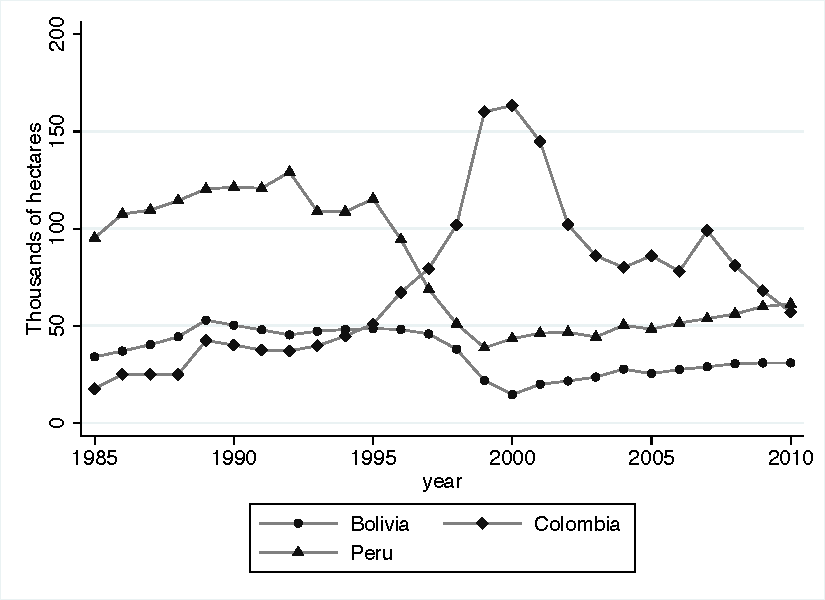
\includegraphics[scale=1]{coca_andean_region.pdf}
	\caption{Presence of coca fields in the Andean region}
	\captionsetup{font={footnotesize}}
	\caption*{Source: Author based on UNODC and U.S. State Department. Estimates for Bolivia include 12,000 hectares authorized since 1988}
	\label{ef_cocaandean}
\end{figure}


\begin{figure}[htbp]
	\centering
	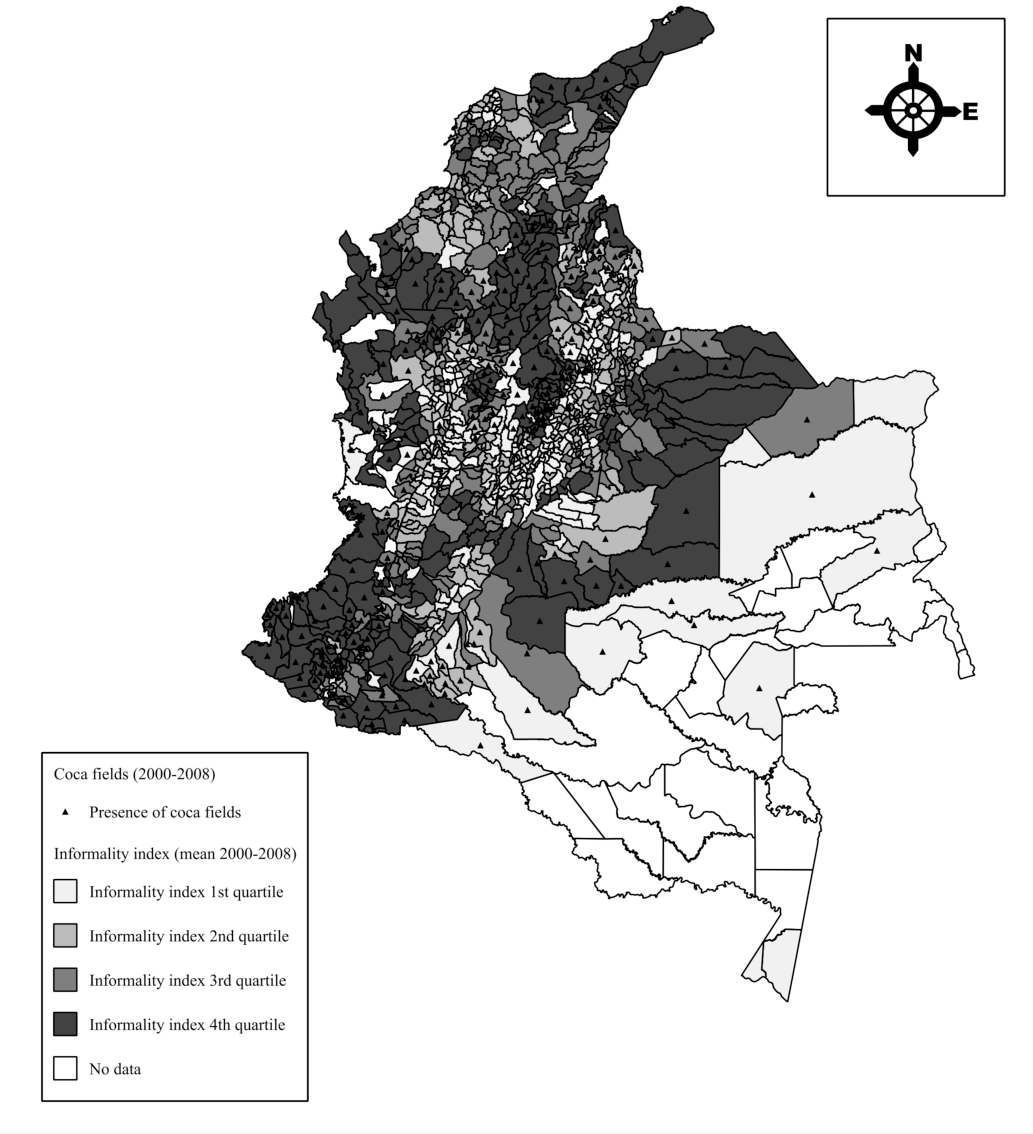
\includegraphics[scale=1]{map_colombia.pdf}
	\caption{Presence of coca fields (any year 2000-2008) and quartiles of informality index (mean 2000-2008) in Colombia}
	\captionsetup{font={footnotesize}}
	\caption*{Source: Author based on UNODC and IGAC. The figure shows municipalities that ever had presence of illicit coca leaf plantations for the period 2000 to 2008 and quartiles of the average informality index for the same period.}
	\label{ds_map}
\end{figure}


\begin{figure}[htbp]
	\centering
	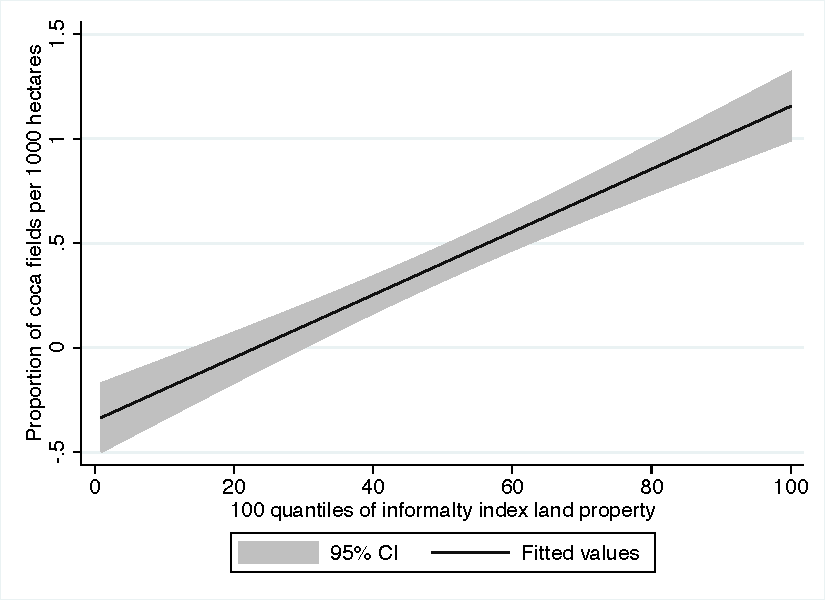
\includegraphics[scale=1]{l_fit.pdf}
	\caption{Linear fit of proportion of coca fields per 1,000 hectares and 100 quantiles of informality index}
	\captionsetup{font={footnotesize}}
	\caption*{Source: Author based on UNODC and IGAC. The linear fit includes 892 municipalities for the period 2000 to 2008.}
	\label{ds_lfit}
\end{figure}

\FloatBarrier
\newpage
\thispagestyle{empty}
\mbox{}\ 